
\documentclass{article}
\usepackage{anyfontsize}
\usepackage[UTF8]{ctex} % 如果需要支持中文
\usepackage{fontspec} 
\usepackage{bookmark}
% \setCJKmainfont{SourceHanSansCN-Light}[
%     BoldFont=SourceHanSansCN-Medium
% ]

\usepackage[a4paper, left=0.1in, right=0.1in, top=0.05in, bottom=0.05in]{geometry} % 设置四边页边距为0.1英寸{geometry} % 设置页边距为0.5英寸
\usepackage{enumitem} % 用于自定义列表
\usepackage{amsmath}  % 数学公式支持

\setlength{\parindent}{0pt} % 不缩进
\usepackage{etoolbox} % 用于列表操作
%调整类代码
\usepackage{comment}
\usepackage{tocloft} % 用于定制目录样式
\usepackage{hyperref} %不需要目录盒子注释这
\usepackage{ifthen}
\usepackage{tikz}
\usepackage{titletoc}
\usepackage{graphicx}
\usepackage{float}
\usepackage{amssymb}  % 提供数学符号，包括\therefore
\usepackage{xcolor}  % 提供颜色支持，用于\textcolor命令
%目录设定
%快捷键 CMD + / 注释
%  \renewcommand{\cftdot}{} % 隐藏目录中的页码
%  \cftpagenumbersoff{section}
%  \cftpagenumbersoff{subsection}
%  \makeatletter
%  \renewcommand{\@pnumwidth}{0em}  % 设置页码宽度为0
%  \renewcommand{\@tocrmarg}{0em}   % 设置右边距为0
%  \makeatother
 
\graphicspath{{images/}}

\usepackage{environ}

\newif\ifshowcontent  % 定义一个条件判断变量
\showcontenttrue    % 设置为 false，隐藏所有 question 环境的内容

\newcounter{question} % 题目计数器
\setcounter{question}{0}
\NewEnviron{question}{%
    \ifshowcontent
    \vspace{1cm}\stepcounter{question}\textbf{\thequestion.} \BODY\par % 如果显示内容，则输出
    \fi
}

\NewEnviron{choices}{%
    \ifshowcontent
        \begin{enumerate}[label=\Alph*., leftmargin=*]
            \BODY
        \end{enumerate}\par
    \fi
}

\NewEnviron{correctanswer}{%
    \ifshowcontent
        \textbf{答案:}\BODY\par
    \fi
}



\newenvironment{explanation}
{\textbf{解析:}\par}
{\par}



% % 新增考察方面命令
% \newcommand{\checklist}[1]{
%     \textbf{考察:} #1 \par % 在题目下方显示考察方面
%     \addcontentsline{toc}{subsection}{题号\thequestion 考察: #1} % 将考察内容添加到目录
%     \vspace{2em} % 添加1em的垂直空间
% }

% \graphicspath{{images/}} %统一







\newcommand{\tocstar}[1]{%
    \texorpdfstring{%
        \protect\textcolor{blue}{%
            \ifnum#1=1 {\protect\textbf{$[\blacksquare\square\square\square\square]$}}\fi%
            \ifnum#1=2 {\protect\textbf{$[\blacksquare\square\square]$}}\fi%
            \ifnum#1=3 {\protect\textbf{$[\blacksquare\blacksquare\square]$}}\fi%
            \ifnum#1=4 {\protect\textbf{$[\blacksquare\blacksquare\blacksquare]$}}\fi%
            \ifnum#1=5 {\protect\textbf{$[\blacksquare\blacksquare\blacksquare\blacksquare\blacksquare]$}}\fi%
        }%
    }{*}%
}



% 在导言区添加以下代码（放在 \begin{document} 之前）
\makeatletter
% 定义新的目录格式
\newcommand{\listbookname}[1]{Book#1 目录}

% 设置目录格式
\renewcommand{\cftsecleader}{\cftdotfill{\cftdotsep}} % 添加虚线
\renewcommand{\cftsecpagefont}{\normalfont}  % 页码字体
\setlength{\cftsecindent}{1em}     % 缩进
\setlength{\cftsecnumwidth}{2.3em}   % 编号宽度
\setlength{\cftbeforesecskip}{1pt}   % 减小节之间的垂直间距

% 为每个book定义新的目录格式
\@for\i:={1,2,3,4}\do{
    \expandafter\newcommand\csname book\i toc\endcsname{\section*{\mdseries\normalfont\listbookname{\i}}}
    \expandafter\newcommand\csname l@book\i\endcsname{\@dottedtocline{1}{1em}{2em}}
}

% 定义四个目录命令
\newcommand{\bookonecontents}{%
    \section*{Foundations of Risk Management 目录}
    \@starttoc{book1}%
}

\newcommand{\booktwocontents}{%
    \section*{Quantitative Analysis 目录}
    \@starttoc{book2}%
}

\newcommand{\bookthreecontents}{%
    \section*{Financial Markets and Products 目录}
    \@starttoc{book3}%
}

\newcommand{\bookfourcontents}{%
    \section*{Valuation and Risk Models 目录}
    \@starttoc{book4}%
}
\makeatother
% 修改 checklist 命令
\newcommand{\checklist}[3]{%
    \textbf{考察:} #1 
    \hspace{1em}
    \textbf{重要程度：}\textcolor{blue}{%
        \ifthenelse{\equal{#2}{1}}{$[\blacksquare\square\square\square\square]$}{%
        \ifthenelse{\equal{#2}{2}}{$[\blacksquare\square\square]$}{%
        \ifthenelse{\equal{#2}{3}}{$[\blacksquare\blacksquare\square]$}{%
        \ifthenelse{\equal{#2}{4}}{$[\blacksquare\blacksquare\blacksquare]$}{%
        \ifthenelse{\equal{#2}{5}}{$[\blacksquare\blacksquare\blacksquare\blacksquare\blacksquare]$}{}}}}}%
    }\par
    \textbf{科目:} \ifthenelse{\equal{#3}{1}}{Foundations of Risk Management}{\ifthenelse{\equal{#3}{2}}{Quantitative Analysis}{\ifthenelse{\equal{#3}{3}}{Financial Markets and Products}{Valuation and Risk Models}}}\par
    % 根据不同的 BOOK 添加到相应的目录
    \ifthenelse{\equal{#3}{1}}{\addcontentsline{book1}{subsection}{题号\thequestion 考察: #1 \tocstar{#2}}}{}
    \ifthenelse{\equal{#3}{2}}{\addcontentsline{book2}{subsection}{题号\thequestion 考察: #1 \tocstar{#2}}}{}
    \ifthenelse{\equal{#3}{3}}{\addcontentsline{book3}{subsection}{题号\thequestion 考察: #1 \tocstar{#2}}}{}
    \ifthenelse{\equal{#3}{4}}{\addcontentsline{book4}{subsection}{题号\thequestion 考察: #1 \tocstar{#2}}}{}
}
% \let\oldtextbf\textbf
% % 重定义 \textbf 命令，使其带有颜色
% \renewcommand{\textbf}[1]{\textcolor{deepblue}{\oldtextbf{#1}}}











\begin{document}
%  %\fontsize{23}{31}\selectfont
%  \tableofcontents % 添加目录
% \newpage
% %\pagestyle{empty}

  % 在需要显示目录的位置添加
  \bookonecontents
  \newpage
  \booktwocontents
  \newpage
  \bookthreecontents
  \newpage
  \bookfourcontents
  
      \newpage
  
  
  \newpage
  
  


\begin{figure}[h]
    \centering
    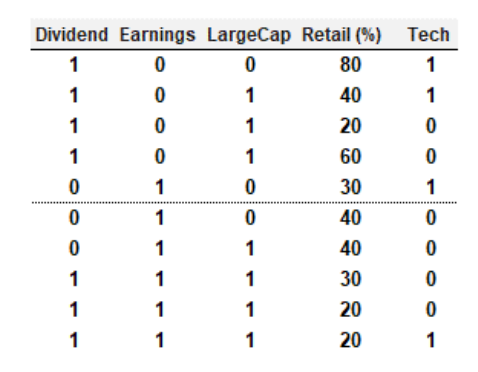
\includegraphics[width=0.8\textwidth]{1·2.png}
\end{figure}





\begin{question}
    Case studies that feature financial engineering by way of complex derivatives include Bankers Trust, the Orange County case, and Sachsen Landesbank. In regard to these financial engineering cases, each of the following statements is true EXCEPT which is false?
\end{question}
    
    \begin{choices}
        \item Bankers Trust (BT) proposed an overly complex swap to their clients (P\&G and Gibson
        Greetings) but the swaps experienced colossal losses; the clients sued BT, who never
        recovered from the ensuing reputational damage
        
        \item  Orange County's treasurer (Robert Citron) borrowed through the repo market to
        purchase inverse floating-rate notes–positions that Citron later said he did not understand–
        but the combination of excessive leverage and embedded interest-rate risk generated losses
        that ultimately forced Orange County to file for bankruptcy
        
        \item Sachsen Landesbank set up off-balance-sheet vehicles (guaranteed by Sachsen) that
        held highly-rated U.S. mortgage-backed securities; the operation was highly profitable, but
        the 2007-08 subprime crisis wiped out Sachsen's capital
        
        \item  If the purpose of the position is designated as hedging (rather than speculation) and if
        the hedge consists only of some combination(s) of forwards, swaps and/or options–which are
        the primary building blocks–then the firm can avoid problems suffered by the financial
        engineering case studies because the firm avoids undue sophistication
        
    \end{choices}
    
    \begin{correctanswer}
    D
    \end{correctanswer}
    
    \begin{explanation}

    \textbf{D选项错误。}
    \begin{itemize}
        \item A hedge does not avoid the assumption of embedded risks that may not be understood; the hedge/speculation intention is important but does not completely warranty the risks of the position. More importantly, complex positions are combinations of the primary building blocks such that complex hedge positions do not avoid running significant
    \end{itemize}
    
    \end{explanation}
    
 \checklist{偿付能力II对保险公司的资本要求}{3}{4}






 \begin{question}
    A very small sample of 10 public companies has one target variable (i.e., Dividend) and four features (i.e., Earnings, LargeCap, Retail, and Tech). Both Dividend and Earnings are binary variables where respectively, one (1) indicates the company recently paid a dividend, and its
    earnings dropped in the previous year. The data frame is displayed below.
    \begin{figure}[H]
        \centering
        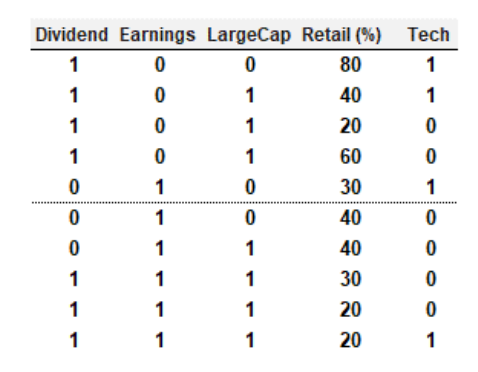
\includegraphics[width=0.3\textwidth]{1·2.png}
    \end{figure}
    Based on Dividend as the output (aka, target) variable, the base Gini coefficient is 0.420. That's because $1- [(7/10)^2 + (3/10)^2]$. What is the information gain if we split (as the root node's feature) the Earnings feature?
    \end{question}
    
    \begin{choices}
        \item Zero
        
        \item 0.120
        
        \item 0.348
        
        \item 0.875
    \end{choices}
    
    \begin{correctanswer}
    B
    \end{correctanswer}
    
    \begin{explanation}

    
    \textbf{B选项正确。}
    \begin{itemize}
        \item We need the weighted Gini coefficient for (splitting on) the Earnings feature. The four {Earnings=0} all pay dividends: this branch is
        pure with a Gini of zero! The Gini of the six {Earnings = 1} branch, where 3 pay dividends and 3 do not, is given by $1 – (3/6)^2 – (3/6)^2$
        = 0.50. The weighted Gini is, therefore, 0*4/10 + 0.50*6/10 = 0.30. The information gain is 0.120 because splitting on the Earnings
        feature reduces from the base Gini of 0.420 to 0.300.
    \end{itemize}
    
    \end{explanation}
    
 \checklist{偿付能力II对保险公司的资本要求}{3}{3}




 \begin{question}
    About swaps, each of the following is true EXCEPT which is false?
    \end{question}
    
    \begin{choices}
        \item At any given time during the life of a bilateral OTC swap, at least one of the
        counterparties incurs both market and credit risk
        
        \item A difference between the typical interest rate swap and currency swap is whether the principal (aka, notional principal) is exchanged
        
        
        \item  Both overnight indexed swaps (OIS) and volatility swaps need to determine a realized (aka, actual) financial variable at the end of a period or tenor
        
        \item A commercial bank funded by short-term floating-rate deposits that extends longterm fixed-rate loans can hedge market risk by entering a swap where it is the floating-rate payer and fixed-rate receiver
    \end{choices}
    
    \begin{correctanswer}
    D
    \end{correctanswer}
    
    \begin{explanation}

 
    \textbf{D选项正确。}
    \begin{itemize}
        \item This is the opposite of a hedge! The bank hedges with a swap where it is the floating-rate receiver and fixed-rate payer In regard to (A), (B), and (C), each is TRUE
    \end{itemize}
    
    \end{explanation}
    
 \checklist{偿付能力II对保险公司的资本要求}{3}{3}




 \begin{question}
    A large international bank uses EWMA for their risk system, with a decay factor of 0.92. On day T the forecast volatility for two variables,
    X\&Y, are identical at 1.25 and the current correlation forecast is 15.0. If on day T the realized returns for X \& Y are 0.50 and -0.50 respectively, which of the following is closest to the new correlation?
    \end{question}
    
    \begin{choices}
        \item  12.5\%
        
        \item 13.4\%
        
        \item 15.0\%
        
        \item  16.2\%
    \end{choices}
    
    \begin{correctanswer}
    B
    \end{correctanswer}
    
    \begin{explanation}

    
    \textbf{A选项错误。}
    \begin{itemize}
        \item 12.5\% is the answer if we use yesterday’s volatilities in the correlation equation

    \end{itemize}
    
    \textbf{B选项错误。}
    \begin{itemize}
        \item Recall the EWMA equations for variance and covariance:
        
        \begin{figure}[H]
            \centering
            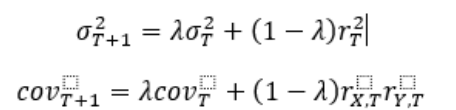
\includegraphics[width=0.3\textwidth]{1·4.png}
        \end{figure}
        
        So, the covariance forecast for day T is $0.15 \times 0.0125 \times 0.0125 = 2.34 \times 10^{-5}$.

        We need to update the variance estimates for X \& Y \& cov(X,Y):

        $\text{Variance}(X) = 0.92 \times (0.0125^2) + (0.08) \times (0.005^2) = 0.00014575$, $\text{Std}(X) = 1.21\%$.

        $\text{Variance}(Y) = 0.92 \times (0.0125^2) + (0.08) \times (-0.005^2) = 0.00014575$, $\text{Std}(Y) = 1.21\%$.

        $\text{Cov}(X,Y) = 0.92 \times (2.34 \times 10^{-5}) + 0.08 \times (0.005) \times (-0.005) = 1.956 \times 10^{-5}$.

        $\text{Corr}(X,Y) = \text{Cov}(X,Y)/(\text{Std}(X) \times \text{Std}(Y)) = 13.4\%$.
    \end{itemize}
    
    \textbf{C选项错误。}
    \begin{itemize}
        \item 15.0\% is the incumbent correlation
    \end{itemize}
    
    \textbf{D选项正确。}
    \begin{itemize}
        \item 16.2\% is the value if use 0.5\% instead of 0.05\% for the return on Y
    \end{itemize}
    
    \end{explanation}
    
 \checklist{偿付能力II对保险公司的资本要求}{3}{3}



 \begin{question}
    According to GARP, each of the following was a causal factor in the 2007-2009 global financial crisis (GFC) EXCEPT which is not a causal factor?
    \end{question}
    
    \begin{choices}
        \item  Low interest rates
        
        \item The originate-to-distribute (OTD) business model and securitization, especially CDOs
        
        \item An unexpected spike in prepayments due to an acceleration in repeat refinancing

        
        \item Dubious lending practices and risky mortgage loan products (e.g., NINJA) and loan features (e.g., teaser rates)
    \end{choices}
    
    \begin{correctanswer}
    C
    \end{correctanswer}
    
    \begin{explanation}

    
    \textbf{A选项错误。}
    \begin{itemize}
        \item Low interest rates (note the dual role in terms of housing demand and investor supply): “Growth in housing demand
        and concomitant mortgage financing was fueled (in part) by the low-interest-rate environment that existed in the
        early 2000s. This demand helped drive substantial increases in housing prices. Low interest rates also spurred investors,
        including institutional investors, to look for investments that offered yield enhancement. They found this yield in
        subprime mortgages, which typically carry premiums of up to 300-basis points over the rates charged to prime
        borrowers.” — Source: 2020 FRM Part I: Foundations of Risk Management, 10th Edition

    \end{itemize}
    
    \textbf{B选项错误。}
    \begin{itemize}
        \item The shift toward banks’ originate-to-distribute (OTD) business model which enabled a moral hazard by discouraging careful scrutiny of borrower creditworthiness.
    \end{itemize}
    
    \textbf{C选项正确。}
    \begin{itemize}
        \item Refinancing enabled borrowers to avoid higher interest rates (as the reset rate) after their initial, teaser rates; the
        PROBLEM was that home price declines halted the refinance practice that fueled much of the subprime borrowing. In this way,
        prepayments were not really a cause.
        In regard to (A), (B) and (D), each is TRUE. Although there were several causes (some disputed), according to GARP’s Chapter 10,
        causal factors included:
        
    \end{itemize}
    
    \textbf{D选项错误。}
    \begin{itemize}
        \item Risky mortgage loan products, in particular, teaser rates; e.g., 2/28 adjustable-rate mortgages. (But also interest-only teaser periods and other “innovations” like NINJA loans).
    \end{itemize}
    
    \end{explanation}
    
 \checklist{偿付能力II对保险公司的资本要求}{3}{3}






\begin{question}
    A hedge fund’s big data algorithm can predict the market’s direction on five out of eight days (62.5\%). Each day’s prediction is either a
    success (e.g., market goes up and algo predicts up) or a failure (e.g., market goes down but algo predicts up). If we dubiously assume the
    predictions are independent, the binomial distribution fits a series of daily predictions over, say, a week or a month. Over two months, the
    probability of each day’s predication being successful, p, equals 5/8 or 62.5\% and the number of days, n, equals 60. We observe that n*p =
    60*62.5\% = 37.5 and n*(1-p) = 60*37.5\% = 22.5, and both of these values (i.e., 37.5 and 22.5) are greater than 10; this satisfies a conventional
    test that says we can use the normal to approximate the binomial. For example, if p were only 1.0\%, then n*p = 6, but 6 is less than 10, and
    such a binomial is deemed to be too skewed to be approximated by the normal distribution. But ours passes the test so we will
    approximate with the normal distribution. If we do rely on the normal distribution to approximate this binomial where p = 5/8 and n = 60,
    what is the probability that the algo makes a correct prediction on only half the days or worse; i.e., where X is the number of successful
    predictions and we approximate with the normal distribution, what is the Pr(X <= 30)?
    \end{question}

\begin{choices}
    \item 2.2750\%
    
    \item 8.3500\%
    
    \item 11.090\%
    
    \item 14.6667\%
\end{choices}

\begin{correctanswer}
    A
    \end{correctanswer}
    
    \begin{explanation}

    \textbf{A选项正确。}
    \begin{itemize}
        \item The variance = $n \times p \times (1-p)$ and the standard deviation = $\sqrt{n \times p \times (1-p)}$; in this case, the standard deviation = $\sqrt{60 \times (5/8) \times (3/8)} = 3.750$. Where $Z = (30 - 60 \times 5/8)/3.750 = -2.0$, the $\Pr(Z < -2.0) = 2.2750\%$.
    \end{itemize}

    \end{explanation}




\begin{question}
    Suppose that it is known that a bond will be delivered in 180 days under the terms of a futures contract. The timing of coupon payments is shown below. The last coupon on the bond was paid 76 days ago, and the next coupon will be paid in 108 days. The coupon after the next one will be paid in 290 days (i.e., 110 days after delivery). Here is the timeline: next one will be paid in 290 days (i.e., 110 days after delivery). Here is the timeline:
\begin{figure}[H]
\centering
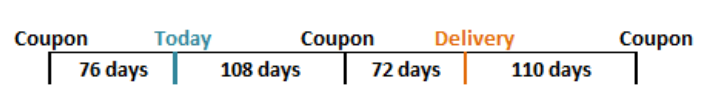
\includegraphics[width=0.5\textwidth]{1·7·1.png}
\end{figure}
    Assume that the risk-free interest rate for all maturities is 5.0\% with continuous compounding and that the delivered bond pays a coupon of 9.0\% semi-annually with a current quoted (clean) price of USD 124.80 and a conversion factor of 1.300.
    Which of the following is nearest to the quoted futures price?
    \begin{choices}
        \item \$95.00
        
        \item \$98.22
        
        \item \$123.50
        
        \item \$125.27
    \end{choices}
\begin{correctanswer}
    A
    \end{correctanswer}
    
    \begin{explanation}

    \textbf{A选项正确。}
   \begin{figure}[H]
    \centering
    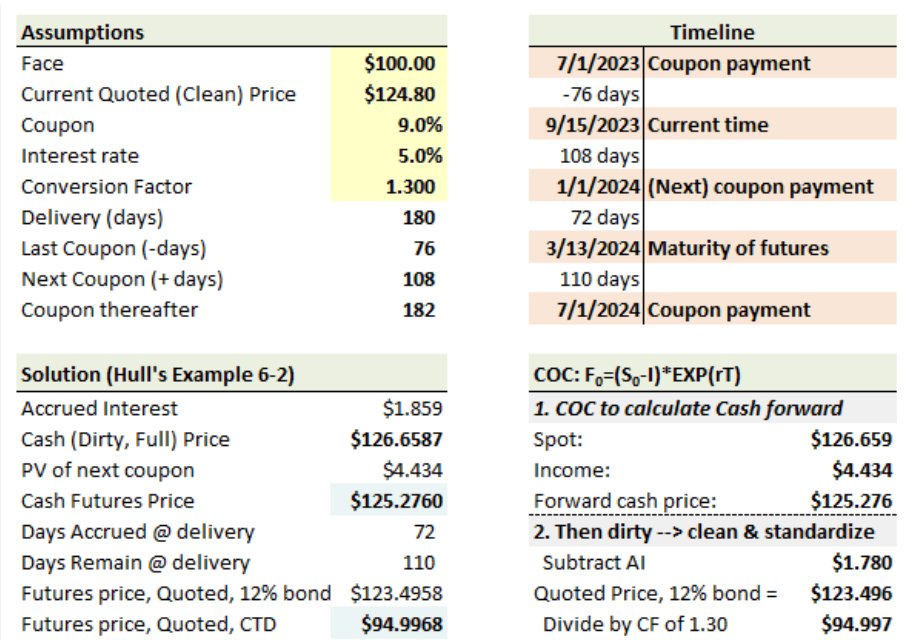
\includegraphics[width=0.5\textwidth]{1·7·2.png}
   \end{figure}
    \end{explanation}
    \end{question}


\begin{question}
    A risk analyst is using the EWMA model to build a daily update of correlation and covariance rates. The two variables are random and are called X and Y. The most recent covariance weight (aka, lambda in the EWMA model) from day n-1 is 0.7. The correlation between X and Y on day N-1 is estimated to be 0.55. X and Y had estimated standard deviations of 0.015 and 0.017 with percentage changes of 3\% and 4\% respectively on day N-1. The updated covariance between X and Y on day n is nearest to which of the following?
    \end{question}

    \begin{choices}
        \item  1.48 $\times$ 10$^{-4}$
        
        \item  4.58 $\times$ 10$^{-4}$
        
        \item 1.18437
        
        \item 0.04581
    \end{choices}


\begin{correctanswer}
    B
    \end{correctanswer}
    
    \begin{explanation}
    \textbf{B选项正确。}
    \begin{itemize}
        \item We can find the EWMA using the following formula:

        $Cov_N = \lambda \times Cov_{N-1} + (1-\lambda) \times X_{n-1} \times Y_{n-1}$

        $\lambda$ = weight of the most recent covariance on day $n-1$

        $X$ = percentage change for variable $X$ on day $n-1$

        $Y$ = percentage change for variable $Y$ on day $n-1$

        We know that $Cov_{xy} = \rho_{xy} \times \sigma_x \times \sigma_y$

        $Cov(n-1) = 0.55 \times 0.015 \times 0.017 = 0.00014025$

        $Cov_N = 0.7 \times 0.00014025 + (1-0.7) \times 3\% \times 4\% = 0.000458175 = 4.58 \times 10^{-4}$
    \end{itemize}
    \end{explanation}



\begin{question}
    Which of the following is TRUE about the SWIFT (Society for Worldwide Interbank Financial Telecommunication) case study?
\end{question}

    \begin{choices}
    \item The 2015-16 cyber-attack (aka, hack) demonstrated that the SWIFT network was unreliable, and it was subsequently phased out
    \item The 2015-16 cyber-attack (aka, hack) successfully exploited vulnerabilities to achieve the theft of about USD 81.0 million
    \item  The 2015-16 cyber-attack (aka, hack) was an unsuccessful attempt to steal money, and it demonstrated the SWIFT network is essentially impervious to attacks
    \item The 2015-16 cyber-attack (aka, hack) was a fictitious news account but the negative press nonetheless shook confidence sufficiently in the network that transactions ground to a halt for several weeks
    \end{choices}
 \begin{correctanswer}
    B
    \end{correctanswer}
    
    \begin{explanation}
    \textbf{B选项正确。}
    \begin{itemize}
        \item The 2015-16 cyber attack (aka, hack) successfully exploited vulnerabilities to achieve the theft of about USD 81.0 million. In regard to (A), (B), and (D), each is FALSE.
    \end{itemize}
    \end{explanation}



\begin{question}
    A credit portfolio contains some number of independent credit-sensitive assets with identical default probabilities; as the defaults are i.i.d., we can use the binomial distribution to characterize the number of defaults. We are told the expected number of defaults is 4.0 with a variance of 3.80. Which is nearest to the probability of exactly four defaults; Pr(X = 4 | binomial with mean of 4.0 and variance of 3.80)?
    \end{question}

    \begin{choices}
        \item Less than 0.01\%
        
        \item 10.0\%
        
        \item  20.0\%
        
        \item 33.3\%
    \end{choices}

    \begin{correctanswer}
     C
    \end{correctanswer}

    \begin{explanation}
    \textbf{C选项正确。}
    \begin{itemize}
        \item The mean of a binomial equals $p \times n$ and the variance equals $p \times (1-p) \times n$. We are told that $p \times n = 4.0$ and $p \times (1-p) \times n = 3.80$. We can
        substitute the first into the second, and thereby determine the number of credits in the portfolio and the default probability:
        If $p \times (1-p) \times n = [p \times n] \times (1-p) = 3.80$, and $p \times n = 4.0$, then $[p \times n] \times (1-p) = 4.0 \times (1-p) = 3.80$, and $p = 1 - \frac{3.80}{4.0} = 5.0\%$.
        Therefore, since $n \times p = 4.0$, $n = \frac{4}{0.050} = 80$.
        The $\Pr(X = 4) = \text{BINOM.DIST}(4, 80 \text{ trials}, 0.050, \text{false}) = 20.043\%$.
    \end{itemize}

    \end{explanation}



    \begin{question}
        At the request of his boss at a large commercial bank, Jason is using the bank's internal model to perform a valuation of a freshly constructed pass-through mortgage-backed security (MBS) pool. The pool contains about 500 mortgages with a principal value of \$400 billion; all of the mortgages originated within the last 30 days. The pool's weighted average coupon (WAC) is 7.50\%. Jason is going to assume a PSA rate of 140\%. This multiplies by 1.40 the baseline 100\% PSA rate that starts at 0.20\% CPR each month for 30 months, then levels at 6.0\% CPR. Each of the following is true EXCEPT which is false?
    \end{question}
    
    \begin{choices}
        \item The pass-through security will pay investors a coupon rate less than 7.50\%
        
        \item The pool factor declines over time due to both scheduled and unscheduled prepayments
        
        \item An increase in the assumption for the PSA rate (e.g., 140\% to 170\%) implies an increase in present value of this pool
        
        \item The single month mortality (SMM) rate excludes scheduled prepayments, and after three years, it will be about 0.7285\%
        
    \end{choices}
    
    \begin{correctanswer}
        C
    \end{correctanswer}
    
    \begin{explanation}
        \textbf{C选项错误。} 
        
        Instead, an increase in the PSA rate models an increase in unscheduled prepayments, which DECREASES the value of the MBS pool.
        
        In regard to (A), (B), and (D), each is TRUE. Specifically,
        \begin{itemize}
            \item The pass-through security will pay investors a coupon rate less than 7.50\%
            \item The pool factor declines over time due to both scheduled and unscheduled prepayments
            \item The single month mortality (SMM) rate excludes scheduled prepayments, and after three years, it will be about 0.7285\%
        \end{itemize}
        
    \end{explanation}

    \begin{question}
        Scott, a risk manager at a small deep-value strategy, is trying to ensure his company is using a coherent risk benchmark. The deep value strategy can be volatile, and thus, Scott wants to see how his capital at risk would adjust if the portfolio had the same holdings but in a smaller proportion to increase its allocation to the risk-free asset. Which principal of a coherent benchmark is reflected in the below scenario?
        
        \begin{table}[H]
            \centering
            \begin{tabular}{|l|c|c|}
                \hline
                \textbf{Portfolio} & \textbf{Scenario 1} & \textbf{Scenario 2} \\
                \hline
                Portfolio & \$20,000,000 & \$20,000,000 \\
                \hline
                Risk-free Allocation & 1.0\% & 11.0\% \\
                \hline
                Risky Allocation & \$19,800,000 & \$17,800,000 \\
                \hline
                Volatility & 24.49\% & 24.49\% \\
                \hline
                Capital at Risk & \$4,850,000 & \$4,360,101 \\
                \hline
                Risk free Capital & \$200,000 & \$2,200,000 \\
                \hline
                Net Capital at Risk & \$4,650,000 & \$2,160,101 \\
                \hline
            \end{tabular}
        \end{table}
    \end{question}
    
    \begin{choices}
        \item Translation Invariance
        
        \item Homogeneity
        
        \item Subadditivity
        
        \item Monotonicity
        
    \end{choices}
    
    \begin{correctanswer}
        A
    \end{correctanswer}
    
    \begin{explanation}
        \textbf{A选项正确。} 
        \begin{itemize}
            \item translation invariance says the addition of (n) reduces the additional cash required by (n). Put more simply, adding cash reduces the risk. For the above example, the increase in the risk-free allocation reduced the risky allocation. The capital at risk was then reduced by the risk-free allocation.
        \end{itemize}
        
        \textbf{B选项错误。}
        \begin{itemize}
            \item  homogeneity refers to the property that multiplying the portfolio size by a constant results in a proportional change in the risk measure.
        \end{itemize}
        
        \textbf{C选项错误}
        \begin{itemize}
            \item  subadditivity states that the sum of two or more portfolios is less than or equal to the sum of their individual risk measures. Adding more assets or asset classes (like commodities) to the portfolio should result in an overall risk measure that is less than or equal to the sum of the individual risk measures.  
        \end{itemize}
        
        \textbf{D选项错误}
        \begin{itemize}
            \item monotonicity implies that if one portfolio has a larger or equal risk than another, then it should also have a larger or equal risk measure. It ensures that adding more assets or increasing allocations to existing assets doesn't increase the risk measure.
        \end{itemize}
        
    \end{explanation}




    \begin{question}
        Barbara is a certified FRM who previously generated income statement and profit projections over a five-year horizon in response to her client's request. Subsequent to the coronavirus outbreak, her client asks Barbara to generate revised financial projections (income statement and balance sheet) and provide the best single point estimate of future revenue, profit, and equity. Barbara utilizes Monte Carlo simulation. Although her client has asked for a single point estimate of these future financial metrics, Barbara perceives that the virus (and the consequential responses) render economic predictions extremely difficult and necessarily laced with great uncertainty. Which of the following is probably her BEST approach to the problem?
    \end{question}
    
    \begin{choices}
        \item She can comply by simply selecting the most probable future outcome; the Code has generally nothing to say about this technical task
        
        \item She can comply but she should qualify her findings to avoid overstating the accuracy of her projections; for example, she can plot a future distribution
        
        \item She should work hard to generate the most precise estimate possible; for example, "sales will go down by 10.85\%" is more useful than "sales will go down by 10\%"
        
        \item She should avoid the temptation to offer any revised future estimates in the face of several "unknown unknowns" because some future values cannot be estimated with sufficient accuracy
        
    \end{choices}
    
    \begin{correctanswer}
        B
    \end{correctanswer}
    
    \begin{explanation}
        \textbf{B选项正确。} She can comply, but she should qualify her findings to avoid overstating the accuracy of her projections; for example, she can plot a future distribution.
        
        According to (4.) Fundamental Responsibilities, GARP Members:
        \begin{itemize}
            \item[4.1] Shall comply with all applicable laws, rules, and regulations (including this Code) governing the GARP Members' professional activities and shall not knowingly participate or assist in any violation of such laws, rules, or regulations.
            \item[4.2] Shall have ethical responsibilities and cannot out-source or delegate those responsibilities to others.
            \item[4.3] Shall understand the needs and complexity of their employer or client and should provide appropriate and suitable risk management services and advice.
            \item[4.4] Shall be diligent about not overstating the accuracy or certainty of results or conclusions.
            \item[4.5] Shall clearly disclose the relevant limits of their specific knowledge and expertise concerning risk assessment, industry practices, and applicable laws and regulations.\textsuperscript{[1]}
        \end{itemize}
        
       
    \end{explanation}





    \begin{question}
        Consider the probability mass function (pmf) below. For example, Pr(X = -1.0) = 20.0\%. 
        \begin{figure}[H]
         \centering
         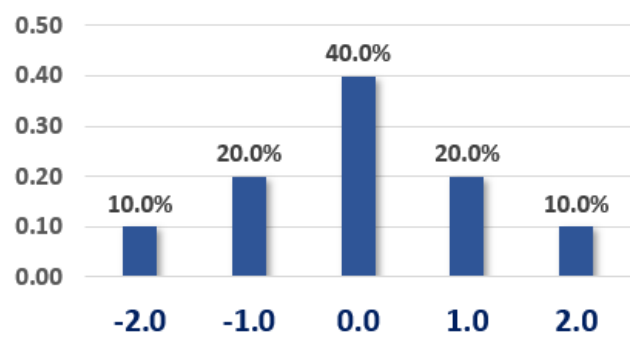
\includegraphics[width=0.4\textwidth]{1·14.png}  
        \end{figure} 
           
        As we can see, this distribution is symmetrical, so we know that its skewness is zero without performing any calculations. We are told the variance is 1.20 (although we can calculate the variance). What is this distribution's kurtosis?
    \end{question}
    
    \begin{choices}
        \item Zero
        
        \item 2.50
        
        \item 3.60
        
        \item 4.40
        
    \end{choices}
    
    \begin{correctanswer}
        B
    \end{correctanswer}
    
    \begin{explanation}
        \textbf{B选项正确。} 
        
        $(-2)^4 \times 10.0\% + (-1)^4 \times 20.0\% + 0^4 \times 40.0\% + 1^4 \times 20.0\% + 2^4 \times 10.0\% = 3.60$, but we need to standardize such that kurtosis = $3.60 / 1.20^2 = 2.50$.
        
        Kurtosis is the fourth central moment (aka, fourth moment about the mean) standardized by the standard deviation raised to the fourth power (aka, square of the second moment). So, in the numerator we have $E[X - \mu(x)]^4$, which is the fourth central moment; and this is divided by $\sigma(X)^4$ in order to standardize the moment. See \url{https://en.wikipedia.org/wiki/Standardized_moment}
        
    \end{explanation}




    \begin{question}
        A U.S. corporate bond that matures on April 1st, 2026, pays a semi-annual coupon of 9.0\% per year. The coupon payment dates are Jan 1st and July 1st. Settlement is on April 7th, 2024. The year 2024 is a leap year. The bond's yield happens to be about 7.00\%. If the cash (aka, dirty) price is \$1,064.50, then which is nearest to the quoted (aka, clean) price? (Inspired by GARP EOC PQ 17.13)
    \end{question}
    
    \begin{choices}
        \item \$960.14
        
        \item \$974.50
        
        \item \$1,040.50
        
        \item \$1,088.50
        
    \end{choices}
    
    \begin{correctanswer}
        C
    \end{correctanswer}
    
    \begin{explanation}
        \textbf{C选项正确。} True: \$1,040.50
        
        On a 30/360 basis, there are $30 \times 3 + 6 = 96$ days. The accrued interest (AI) is $\$1,000 \times 9.0\%/2 \times 96/180 = \$24.00$.
        
        Therefore, the bond's quoted price is $\$1,064.50 - 24.00 = \$1,040.50$.
        
        Please note we could have retrieved the cash price (which is given) by starting with the bond price at the last coupon date; \$1,045.151 is the price of the bond on 1/1/2024 where $N=5$, $I/Y=3.5\%$, $PMT=45$, and $FV = 1,000$. Then compounded forward: $\$1,045.151 \times (1+7.0\%/2)^{96/180} = \$1064.50$.
        
    \end{explanation}



    \begin{question}
        When is the soonest that an obligation rated AAA (the highest rating) can default?
    \end{question}
    
    \begin{choices}
        \item During the first year (i.e., by the end of the first year) with a margin probability of 2.0\%
        
        \item During the second year (i.e., between the end of the first and second year) with a joint probability of 0.1879\% (or 0.001879 or $1.879 \times 10^{-3}$)
        
        \item During the third year (i.e., between the end of the second and third year) with an unconditional probability of 0.00540\% (or 0.0000540 or $5.40 \times 10^{-5}$)
        
        \item During the fourth year (i.e., between the end of the third and fourth year) with a conditional probability of 2.00\%
        
    \end{choices}
    
    \begin{correctanswer}
        C
    \end{correctanswer}
    
    \begin{explanation}
        \textbf{C选项正确。} TRUE: During the third year (i.e., between the end of the second and third year) with an unconditional probability of 0.00540\% (or 0.0000540 or $5.40 \times 10^{-5}$)
        
        At the end of the first year, the worst downgrade (from AAA) is only to AA with a 9.0\% probability. Conditional on the AA-rating at the start of the second year, the worst downgrade possible is to BB with a conditional probability of 3.0\% (if downgraded to BBB or higher, this obligation cannot default by the end of the third year!). Conditional on the BB-rating at the start of the third year, the obligation can default during the third year with a conditional probability of 2.0\%. The probability is given by $9.0\% \times 3.0\% \times 2.0\% = 0.005400\%$.
        
    \end{explanation}






    \begin{question}
        Arguably the U.S. savings and loan (S\&L) crisis in the 1980s had multiple causes, but among the following which is the BEST summary explanation of the S\&L crisis?
    \end{question}
    
    \begin{choices}
        \item S\&Ls engaged in a practice called "riding the yield curve" but this was one of the central bank's monetary policy tools and was not meant to be performed by private banks
        
        \item The Fed's restrictive monetary policy led to a dramatic increase in short-term interest rates which wiped out bank's interest rate spread due to their asset-liability mismatch
        
        \item The Fed's expansionary monetary policy led to a dramatic decrease in short-term interest rates which wiped out bank's interest rate spread due to their asset-liability mismatch
        
        \item New regulations introduced in the early 1980s hindered the ability of the savings and loan (S\&L) industry to lend and/offer new loan products that could help it grow out of its problems
        
    \end{choices}
    
    \begin{correctanswer}
        B
    \end{correctanswer}
    
    \begin{explanation}
        \textbf{B选项正确。} True: The Fed's restrictive monetary policy led to a dramatic increase in short-term interest rates which wiped out bank's interest rate spread due to their asset-liability mismatch.
        
        As explained by GARP, "However, rising inflation in the late 1970s prompted the Fed to implement a restrictive monetary policy, which led to a significant increase in short-term interest rates. The increase in short-term rates pushed up funding costs for S\&Ls, wiping out the interest rate spread they depended on for their profit margin. The spike in their short-term funding costs (which were needed to finance long-term fixed-interest rate mortgages) meant that S\&Ls generated negative net interest margins on many of their long-term residential mortgage portfolios."\textsuperscript{[1]}
        
        \textsuperscript{[1]} 2020 FRM Part I: Foundations of Risk Management, 10th Edition. Pearson Learning Solutions, 10/2019
        
    \end{explanation}







\begin{question}
    Consider the probability mass function (pmf) below. For example, Pr(X = -1.0) = 20.0\%. The pmf is given by $f(x) = x \times a$. The domain of the variable is the set of integers $\{6, 7, 8, 9, 10\}$. What is the expected value of this discrete random variable?
\end{question}

\begin{choices}
    \item 6.67
    
    \item 8.00
    
    \item 8.25
    
    \item 9.33
    
\end{choices}

\begin{correctanswer}
    C
\end{correctanswer}

\begin{explanation}
    \textbf{C选项正确。} True: 8.25
    
    We know that $6a + 7a + 8a + 9a + 10a = 1.0$ such that $a = 1/40 = 0.0250$ and the pmf is given by $f(x) = x/40 = 0.0250 \times x$.
    
    The expected value equals $1/40 \times (6^2 + 7^2 + 8^2 + 9^2 + 10^2) = 8.25$.
    
\end{explanation}





\begin{question}
    Assume the following six-month forward rates that are quoted per annum with semi-annual compounding:
    \begin{itemize}
        \item $F(0, 0.5) = S(0.5) = 2.0\%$; i.e., the six-month spot rate
        \item $F(0.5, 1.0) = 4.0\%$
        \item $F(1.0, 1.5) = 6.0\%$
    \end{itemize}
    If the price of a 7.0\% semi-annual coupon bond is \$103.20, which is nearest to the 2-year spot rate?
\end{question}

\begin{choices}
    \item 4.30\%
    
    \item 5.40\%
    
    \item 6.60\%
    
    \item 7.90\%
    
\end{choices}

\begin{correctanswer}
    B
\end{correctanswer}

\begin{explanation}
    \textbf{B选项正确。} True: 5.40\%
    
\end{explanation}




\begin{question}
    In regard to through-the-cycle (TTC) versus at-the-point (aka, point in time, PIT) approaches to credit ratings, each of the following statements is true EXCEPT which is false?
\end{question}

\begin{choices}
    \item Agency (i.e., external) credit ratings tend to be through-the-cycle (TTC)
    
    \item Through-the-cycle (TTC) is conditional, while at-the-point (PIT) is unconditional
    
    \item Credit spreads are at-the-point (PIT) and PIT measures incorporate more information
    
    \item During crisis periods, PIT approaches imply higher expected and unexpected loss (EL \& UL) such that PIT tends to be pro-cyclical
    
\end{choices}

\begin{correctanswer}
    B
\end{correctanswer}

\begin{explanation}
    \textbf{B选项错误。} Instead, true is: Through-the-cycle (TTC) is unconditional, while at-the-point (PIT) is conditional.
    
    In regard to (A), (C) and (D), each is TRUE.
    
    \textbf{In regard to true (A),} external agency credit ratings tend to be through-the-cycle (TTC).
    
    \textbf{In regard to true (C),} credit spreads are at-the-point (PIT) and PIT measures theoretically incorporate more information. Please note this point is debatable. Some people would argue that much of the information in some PIT approaches (e.g., structural) contain too much noise masquerading as information.
    
    \textbf{In regard to true (D),} during crisis periods, PIT approaches imply higher expected and unexpected loss (EL \& UL) such that PIT tends to be pro-cyclical.
    
\end{explanation}




\begin{question}
    Alice, Bert, Chris, Don, Eva, and Fred are individual investors. Each of them exhibits a particular behavioral bias.
    \begin{itemize}
        \item Alice (A) invested in the stock Cloudera (CLDR) and bad news (aka, new information) renders her original thesis obsolete but she is reluctant to sell today because an exit implies the realization of a -30.0\% loss on the position and she much prefers to sell after her position experiences a double-digit gain
        \item Bert (B) can buy a new smartphone for \$79.00 but he cannot resist a sale and prefers to pay \$100.00 because it represents a 50.0\% discount from the retail (MSRP) price
        \item Chris (C) attends an investment conference but he avoids the seminar focusing on recession risks because he is overweight homebuilders and he worries the topic will make him anxious with worry
        \item Don (D), who enjoys food shopping, tends to be price-conscious (e.g., he seeks bargains) when he pays cash at Sprouts or Trader Joes, but when he uses his Amazon credit card at Whole Foods he doesn't worry about the cost because he doesn't look at the statement for several days or weeks
        \item Eva (E) purchased Facebook (FB) at \$160.00 because his firm's price target was \$200.00, and he decides to ignore new information until the price reaches this level
        \item Fred (F) was previously a patient buy-and-hold investor who purchased high-conviction stocks and only checked his portfolio once a week, but last year he signed up for a subscription to Seeking Alpha and since that time his buy/sell transactions have quintupled because he's reading news about his portfolio holdings every day
    \end{itemize}
    Which of the following correctly matches the individual investor to his or her behavioral bias?
\end{question}

\begin{choices}
    \item A = Home bias, B = Mental accounting, C = Ostrich effect, D = Herding, E = Groupthink, F = Framing
    
    \item A = Loss aversion, B = Framing, C = Ostrich effect, D = Mental accounting, E = Anchoring, F = Feedback effects
    
    \item A = Groupthink, B = Herding, C = Home bias, D = Framing, E = Loss aversion, F = Ostrich effect
    
    \item A = Mental accounting, B = Home bias, C = Loss aversion, D = Groupthink, E = Feedback effects, F = Herding
    
\end{choices}

\begin{correctanswer}
    B
\end{correctanswer}

\begin{explanation}
    \textbf{B选项正确。} TRUE: A = Loss aversion, B = Framing, C = Ostrich effect, D = Mental accounting, E = Anchoring, F = Feedback effects
    
    According to GARP's Box 8.3:\textsuperscript{[1]}
    \begin{itemize}
        \item \textbf{Anchoring and referencing:} This is the use of mental reference points to contextualize a decision (e.g., such as using an existing price point to determine whether a new price point is attractive or not). The anchor may influence the decision-making process in an irrational way. Furthermore, the various reference points in a collection of related decisions may lack coherence.
        \item \textbf{Feedback effects:} The presence or absence of frequent, positive feedback can irrationally influence the ability of decision-makers to stick to a decision.
        \item \textbf{Framing:} How a choice is framed can push a decision-maker toward one decision or another. For example, a consumer may be willing to hunt for a 50\% savings on a phone case (saving themselves USD 10) but be unwilling to make the same effort to save the USD 10 when buying a USD 200 phone (because it represents a smaller percentage of the purchase price).
        \item \textbf{Groupthink:} This describes the tendency of individuals within groups to overcome their doubts about a risky decision (or keep quiet) in favor of the group consensus. The consensus may itself have been shaped by a dominant individual, poorly set targets, or selective reading of ambiguous evidence.
        \item \textbf{Herding:} Herding is the tendency of investors to copy the actions of others, both when investing and when reducing losses in a volatile market. Herding effects in risk management can lead to too many investors using the same risk metrics or setting the same stop-losses, leading to sharp market sell-offs.
        \item \textbf{Home bias:} This describes the tendency of investors to invest in domestic securities rather than building a globally diversified portfolio, perhaps because of the uncertainties attached to foreign markets.
        \item Loss aversion: Experiments show that for most people the potential for losses outweighs potential gains of similar
        magnitude. This can lead a decision-maker to favor a result that is presented as certain while foregoing the chance of
        larger but riskier wins. Loss aversion does not always lead to conservative risk decisions. It can also encourage decisionmakers to take irrationally risky decisions to preserve some chance of avoiding a loss. (Whether a decision is framed as
        a loss or as a potential gain is also therefore important.)
        \item Mental accounting: People seem to account for money within separate categories that are treated differently as if the
        money was not completely fungible across accounts. For example, consumers might spend more if they use a credit
        card compared to using cash. Investors might invest the money from an inheritance differently than money from a
        gambling win. They may also be reluctant to “close” a mental account if it involves declaring a loss or mistake. Loss
        aversion and other behavioral phenomena, such as the treatment of “sunk” costs, often further distort mental
        accounting.
        \item Ostrich effect: This describes the irrational tendency to avoid observing bad news that might precipitate
        uncomfortable decisions or actions. For example, an investor might pay more attention to booming stock markets
        than flat or falling markets. (Conversely, an investor that pays too much attention to each individual loss can suffer from
        irrational aversion.)
        

        
    \end{itemize}
    
    \textsuperscript{[1]} 2020 FRM Part I: Foundations of Risk Management, 10th Edition. Pearson Learning Solutions, 10/2019
    
\end{explanation}






\begin{question}
    The probability graph below illustrates event A (the yellow rectangle) and event B (the blue rectangle). The unconditional probability of event A is 50.0\% and the unconditional probability of event B is 44.0\%; i.e., $\Pr(A) = 50.0\%$ and $\Pr(B) = 44.0\%$. Their overlap is graphed by the green rectangle such that $\Pr(A \cap B) = 27.0\%$. The orange rectangle conditions on the event C. For example, conditional on event C, there is a 50.0\% probability that event A occurs, $\Pr(A | C) = 50.0\%$.

    \begin{figure}[H]
     \centering
     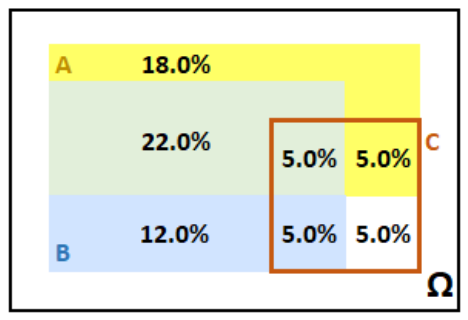
\includegraphics[width=0.4\textwidth]{1·22.png}   
    \end{figure}
   
    Which of the following is TRUE about, respectively, the unconditional and conditional relationship between events A and B?
\end{question}

\begin{choices}
    \item A and B are unconditionally dependent but conditionally (on event C) independent
    
    \item A and B are unconditionally dependent and also conditionally (on event C) dependent
    
    \item A and B are unconditionally independent but conditionally (on event C) dependent
    
    \item A and B are unconditionally independent and also conditionally (on event C) independent
    
\end{choices}

\begin{correctanswer}
    A
\end{correctanswer}

\begin{explanation}
    \textbf{A选项正确。} True: A and B are unconditionally dependent but conditionally (on event C) independent.
    
    If A and B are unconditionally independent, then it must be true that $\Pr(A \cap B) = P(A) \times P(B)$; however, in this case, $P(A) \times P(B) = 50.0\% \times 44.0\% = 22.0\%$, but $\Pr(A \cap B) = 27.0\%$. Therefore, A and B are unconditionally dependent.
    
    On the other hand, A and B are conditionally independent because it is true that $\Pr(A \cap B | C) = \Pr(A | C) \times \Pr(B | C)$. The $\Pr(A \cap B | C) = 5.0\%/20.0\% = 25.0\%$, and $\Pr(A | C) \times \Pr(B | C) = (10.0\%/20.0\%) \times (10.0\%/20.0\%) = 0.50 \times 0.50 = 25.0\%$.
    
\end{explanation}








\begin{question}
    We are told to assume that an interest rate is 9.00\% per annum with quarterly compounding. Each of the following statements is true EXCEPT which is false?
\end{question}

\begin{choices}
    \item The effective annual rate is higher than 9.00\%
    
    \item The equivalent rate with continuous compounding is higher than 9.00\%
    
    \item The equivalent rate with monthly compounding (i.e., 12 periods per year) is lower than 9.00\%
    
    \item The stated (aka, quoted, nominal) rate is given as 9.00\% such that the periodic rate is 2.25\%
    
\end{choices}

\begin{correctanswer}
    B
\end{correctanswer}

\begin{explanation}
    \textbf{B选项错误。} Instead, the equivalent rate with continuous compounding is LOWER than 9.00\%.
    
    In regard to (A), (C), and (D), each is TRUE.
    
    Specifically, if an interest rate is 9.00\% per annum with quarterly compounding, then:
    \begin{itemize}
        \item The equivalent continuous rate is $4 \times \ln(1 + 9\%/4) = 8.90\%$
        \item The equivalent rate with monthly compounding is $[(1 + 9\%/4)^{4/12} - 1] \times 12 = 8.933\%$
        \item The effective annual rate is $(1+9\%/4)^4-1 = 9.3083\%$; i.e., the equivalent rate with annual compounding
    \end{itemize}
    
    If the stated (aka, quoted, nominal) rate is given as 9.00\%, and there are four periods per year (aka, quarterly compounding), then the periodic rate is $9.00\%/4 = 2.25\%$.
    
\end{explanation}


                    





\begin{question}
    Quotecan Corporation has issued a bond. Quotecan's interest coverage ratio is within reasonable limits, providing adequate protection for investors in the near term. The bond is "better than junk" but carries more credit risk than bonds issued by the highest-rated corporations (e.g., Microsoft, Apple, Exxon Mobil, Johnson \& Johnson, and Walmart). Quotecan's capacity to repay may be impaired if adverse economic conditions materialize, or if circumstances suddenly change. While the obligations are not speculative in their entirety, they do contain just a few speculative elements which may render the protective elements unreliable over a longer time horizon. Based on these facts, which credit rating is most likely assigned to Quotecan's bond offering?
\end{question}

\begin{choices}
    \item A-1 or P-1
    
    \item AA or Aa
    
    \item B or B
    
    \item BBB or Baa
    
\end{choices}

\begin{correctanswer}
    D
\end{correctanswer}

\begin{explanation}
    \textbf{D选项正确。} True: BBB (Standard \& Poor's) or Baa (Moody's) rating is most likely; i.e., it is the lowest rating among the investment-grade ratings. See \url{https://en.wikipedia.org/wiki/Credit_rating}.
    
    According to S\&P, an obligation rated "BBB" exhibits adequate protection parameters. However, adverse economic conditions or changing circumstances are more likely to weaken the obligor's capacity to meet its financial commitments on the obligation.
    
    According to Moody's, the rating of "Baa" corresponds to obligations of moderate credit risk that may possess speculative characteristics.
    
\end{explanation}






\begin{question}
    GARP explains that "perhaps the biggest argument for ERM is that an enterprise-level perspective is the best way to prioritize risks and optimize risk management." Each of the following is one of the four key reasons that enterprise risk might demand the practice of (or, the art and science of) enterprise risk management, ERM, EXCEPT which is NOT one of the four key reasons?
\end{question}

\begin{choices}
    \item Identify hidden and/or dangerous concentrations including (for example) geographical, industry, product, or among suppliers
    
    \item Vertical vision recognizes potential threats to the whole enterprise ideally in their early stages to reduce the leverage effect of time
    
    \item Portfolio thinking permits the business units to specify a more accurate distribution that incorporates the allocation of corporate overhead
    
    \item Thinking beyond silos acknowledges diversification among risk types and better understanding of how interactions might worsen enterprise threats
    
\end{choices}

\begin{correctanswer}
    C
\end{correctanswer}

\begin{explanation}
    \textbf{C选项错误。} Instead, the fourth is: translate a better understanding of risks to the enterprise, in particular insurable risks, into costs savings and/or better resource allocation.
    
    The four key reasons why enterprise risk might demand ERM are:
    \begin{itemize}
        \item Identify hidden and/or dangerous concentrations including (for example) geographical, industry, product, or among suppliers
        \item Vertical vision recognizes potential threats to the whole enterprise ideally in their early stages to reduce the leverage effect of time
        \item Translate a better understanding of risks to the enterprise, in particular insurable risks, into costs savings and/or better resource allocation
        \item Thinking beyond silos acknowledges diversification among risk types and better understanding how interactions might worsen enterprise threats
    \end{itemize}
    
\end{explanation}






\begin{question}
    Yesterday a web page hosted by Acme received tens of thousands of page views but some were views by malicious bots. Acme utilizes two software applications to detect these malicious "bot-views." It uploads the same data file from yesterday to both applications. The first application detects 200 bot-views and the second application detects 300 bot-views. Among these, only 40 bot-views were detected by both applications. All bot-views are equally likely to be located, but clearly both applications only identify a minority of the bot-views (otherwise there would be a much higher number of identified bot-views common to both applications). Further, the identification of a bot-view by one application is independent of its identification by the other application. How many malicious bot-views did the web page experience on this day?
\end{question}

\begin{choices}
    \item 300
    
    \item 460
    
    \item 540
    
    \item 1,500
    
\end{choices}

\begin{correctanswer}
    D
\end{correctanswer}

\begin{explanation}
    \textbf{D选项正确。} True: 1,500
    
    The second application identified $40/200 = 20.0\%$ of those identified by the first application, therefore (per the independence), we can infer that its own 300 identifications is about $20.0\%$ of the total number such that we estimate $300/20\% = 1,500$ total bot-views. Similarly, the first application identified $40/300 = 13.33\%$ of those identified by the second application, so we can infer that its own 200 identification represents about $13.33\%$ of the total, which is also $200/13.33\% = 1,500$.
    
\end{explanation}



\begin{question}
    Consider a binary cash-or-nothing call option that pays \$100.00 if the stock is above \$100.00 at maturity in three months. The option's underlying non-dividend-paying stock is currently trading at \$85.00. The riskfree rate is 4.0\% per annum with continuous compounding. We are also told that while $S = \$85.00$ and $K = \$100.00$, $N(d_1) = 0.12350$ and $N(d_2) = 0.100$, and the price of a vanilla three-month European call option on this stock is \$0.62. Which is nearest to the price of the cash-or-nothing call?
\end{question}

\begin{choices}
    \item \$0.62
    
    \item \$9.88
    
    \item \$10.50
    
    \item \$20.38
    
\end{choices}

\begin{correctanswer}
    B
\end{correctanswer}

\begin{explanation}
    \textbf{B选项正确。} True: \$9.88
    
    $\$100.00 \times 0.10 \times \exp(-4.0\% \times 0.25) = \$9.88$.
    
    Alternatively, we can retrieve the price of the asset-or-nothing as given by $\$85.00 \times 0.12350 \times \exp(0\% \times 0.25) = \$10.50$ such that $\$10.50 - \$0.62 = \$9.88$.
    
\end{explanation}







\begin{question}
    Rebecca is evaluating four different countries in an attempt to determine their respective default risk. She evaluates the countries in four categories: degree of indebtedness as measured by debt as a percentage of gross domestic product; social service/pension commitments as estimated by the average age of the population; nature of the economy (e.g., diverse versus concentrated in oil as a natural resource), and monetary policy. The four countries are summarized in the exhibit below:
    
    \begin{table}[H]
        \centering
        \begin{tabular}{|l|c|c|c|c|}
            \hline
            \textbf{Country} & \textbf{Debt as \% of GDP} & \textbf{Age of Population} & \textbf{Economy} & \textbf{Monetary Policy} \\
            \hline
            Country A & $>$ 100\% & Old & Diverse & Independent CB \\
            \hline
            Country B & $\sim$ 100\% & Young & Tourism & EU member \\
            \hline
            Country C & 50\% & Young & Oil & Autocracy \\
            \hline
            Country D & 30\% & Old & Diverse & Semi-independent CB \\
            \hline
        \end{tabular}
    \end{table}
    
    Which of the four countries is most likely to default?
\end{question}

\begin{choices}
    \item Country A is the most likely to default because debt above 100\% is highly predictive of default and overwhelms the other indicators
    
    \item Country B is the most likely to default because it is the only country with three (out of four) negative indicators
    
    \item Country C is the most likely to default because it has an autocratic government
    
    \item It is unclear: each has two negative (and two positive) indicators; further, quantification of this scorecard is an insufficient predictor
    
\end{choices}

\begin{correctanswer}
    D
\end{correctanswer}

\begin{explanation}
    \textbf{D选项正确。} It is unclear: each has two negative (and two positive) indicators; further, quantification of this scorecard is an insufficient predictor.
    
    Damodaran: "In summary, a full assessment of default risk in a sovereign entity requires the assessor to go beyond the numbers and understand how the country's economy works, the strength of its tax system and the trustworthiness of its governing institutions."\textsuperscript{[1]}
    
    In regard to (A), (B) and (C), each is not the best answer:
    \begin{itemize}
        \item In regard to (A), Damodaran casts debt as a percentage of GDP as an incomplete measure of default risk. Countries with high debt include Greece, Congo, Jamaica, Egypt (high risk) but also US, Japan, France, Canada (creditworthy).\textsuperscript{[1]} In regard to (B), Country B has only two negative indicators: high debt/GDP and an economy concentrated in tourism. But in regard to Damodaran casts EU membership as net positive: "6. Implicit backing from other entities: When Greece, Portugal and Spain entered the European Union, investors, analysts and ratings agencies reduced their assessment of default risk because of the implicit backing from stronger EU members. This backing is not explicit or legally binding, but it does exist."\textsuperscript{[1]} In regard to (C), Damodaran: "Default is a political decision, and autocracies might be more likely to default because there is less political backlash." However, "The independence and power of the central bank can affect default risk assessments."\textsuperscript{[1]}
    \end{itemize}
    
    \textsuperscript{[1]} 2020 FRM Part I: Foundations of Risk Management, 10th Edition. Pearson Learning Solutions, 10/2019
    
\end{explanation}







\begin{question}
    GARP explains that the Basel Committee on Banking Supervision's standard number 239 (aka, BCBS 239) "was a major driver in the rise of the chief data officer (CDO) function. The CDO is typically responsible for standardizing a firm's approach to data management."\textsuperscript{[1]} In addition, which of the following statements is also TRUE about the Basel Committee on Banking Supervision's standard number 239 (aka, BCBS 239)?
\end{question}

\begin{choices}
    \item BCBS 239 offers the advantage of a uniform blueprint for a compliant IT infrastructure
    
    \item Every systematically important financial institution (SIFI) complied with the original timeline
    
    \item Compliance with BCBS 239 is a subjective exercise and the standards for each bank are bespoke
    
    \item While praised for its theory, critics say BCBS 239 forgets to address risk management data and models
    
\end{choices}

\begin{correctanswer}
    C
\end{correctanswer}

\begin{explanation}
    \textbf{C选项正确。} TRUE: Compliance with BCBS 239 is a subjective exercise and the standards for each bank are bespoke.
    
    In regard to (A), (B) and (D) each is FALSE. Instead, the following are TRUE statements:
    \begin{itemize}
        \item "There is no uniform blueprint in place for a BCBS 239-compliant infrastructure and solutions are specific to each institution. The optimal approach ensures that all people and systems within the banking group are working with the same data, the same models, and the same assumptions," explains GARP.\textsuperscript{[1]}
        \item "Banks have struggled to comply with BCBS 239 and the original timeline to achieve full compliance was not met by any bank. This is largely due to the highly complex nature of the IT reengineering involved in bringing the various systems into compliance as well as the dynamic nature of the principles. The exponential increase in the application of AI techniques on large data sets has also made compliance with BCBS 239 more challenging," explains GARP.\textsuperscript{[1]}
        \item While implementation has lagged, BCBS 239 does (at least attempt to) address risk management data and models in a practical way.
    \end{itemize}
    
    \textsuperscript{[1]} 2020 FRM Part I: Foundations of Risk Management, 10th Edition. Pearson Learning Solutions, 10/2019
    
\end{explanation}






\begin{question}
    For her investment firm, Audrey has identified six high-priority machine learning use cases. They are given below in three pairs:
    \begin{itemize}
        \item I. Segment customers into different groups; and perform sentiment analysis of 10K SEC filings
        \item II. Predict if borrower(s) will default; and forecast future stock price(s) based on fundamental data
        \item III. Decide how to split large-volume trades to sell quickly while minimizing the adverse price effect, and decide how much of a position to hedge using derivatives.
    \end{itemize}
    The three top-level machine learning approaches are supervised learning (S), unsupervised learning (U), and reinforcement learning (R).
    Which of the following is the best mapping of the advisable machine learning approach to its corresponding pair of use cases above?
\end{question}

\begin{choices}
    \item SRU: I=Supervised, II=Reinforcement, III=Unsupervised
    
    \item RUS: I=Reinforcement, II=Unsupervised, III=Supervised
    
    \item RUU: I=Reinforcement, II=Unsupervised, III=Unsupervised
    
    \item USR: I=Unsupervised, II=Supervised, III=Reinforcement
    
\end{choices}

\begin{correctanswer}
    D
\end{correctanswer}

\begin{explanation}
    \textbf{D选项正确。} True: USR: I=Unsupervised, II=Supervised, III=Reinforcement
    
    These pairs map as follows:
    \begin{itemize}
        \item I. Unsupervised: Customer segmentation implies clustering, and sentiment analysis implies natural language processing (NLP).
        \item II. Supervised: Default prediction and asset price forecasting are classic applications of supervised learning.
        \item III. Reinforcement: As GARP explains, "Reinforcement learning has many applications in risk management. For example, it is used to determine the optimal way to buy or sell a large block of shares, to determine how a portfolio should be managed, and to hedge derivatives portfolios [section 14.1] \ldots As mentioned earlier, there are also many potential applications in finance, including for technical trading rules, determining how to split large-volume trades to sell quickly while minimizing the adverse price effect, and determining how much of a position to hedge using derivatives." [Section 14.7]
    \end{itemize}
    
\end{explanation}




\begin{question}
    A non-dividend-paying stock has a current price of \$10.00 and a volatility of 25.0\% per annum. The risk-free rate is 4.0\% per annum with continuous compounding. Consider the following four spread trades:
    \begin{itemize}
        \item Trade \#1 is a bull spread with calls. The strike prices are: $K_1 = \$9.00$, $K_2 = \$11.00$. The up-front cost is \$1.00.
        \item Trade \#2 is a bull spread with puts. The strike prices are: $K_1 = \$9.00$, $K_2 = \$11.00$. The up-front cash flow is \$0.93.
        \item Trade \#3 is a bear spread with puts. The strike prices are: $K_1 = \$8.00$, $K_2 = \$12.00$. The up-front cost is \$1.84.
        \item Trade \#4 is a bear spread with calls. The strike prices are: $K_1 = \$8.00$, $K_2 = \$12.00$. The up-front cash flow is \$2.00.
    \end{itemize}
    In regard to each trade's maximum profit, each of the following statements is true EXCEPT which is false?
\end{question}

\begin{choices}
    \item Trade \#1 offers a maximum profit of \$1.00
    
    \item Trade \#2 offers a maximum profit of \$0.93
    
    \item Trade \#3 offers a maximum profit of \$0.84
    
    \item Trade \#4 offers a maximum profit of \$2.00
    
\end{choices}

\begin{correctanswer}
    C
\end{correctanswer}

\begin{explanation}
    \textbf{C选项错误。} Instead, Trade \#3 offers a maximum profit of \$2.16. In regard to (A), (B), and (D), each is TRUE.
    
\end{explanation}





\begin{question}
    Political Risk Services (The PRS Group) provides numerical measures of country risk for more than a hundred countries. Its International Country Risk Guide (ICRG) rating "comprises 22 variables in three subcategories of risk: political, financial, and economic. A separate index is created for each of the subcategories. The Political Risk index is based on 100 points, Financial Risk on 50 points, and Economic Risk on 50 points. The total points from the three indices are divided by two to produce the weights for inclusion in the composite country risk score."\textsuperscript{[1]}
    
    As of July 2018, according to Damodaran, Taiwan's composite (ICRG) score was 85. Which of the following is TRUE?
\end{question}

\begin{choices}
    \item Taiwan is very low risk
    
    \item This score is irrelevant for investment purposes
    
    \item This score can be neither normalized nor standardized
    
    \item This score cannot be used to rank Taiwan against other countries
    
\end{choices}

\begin{correctanswer}
    A
\end{correctanswer}

\begin{explanation}
    \textbf{A选项正确。} TRUE: Taiwan is very low risk. The composite scores, ranging from zero to 100, are then broken into categories from Very Low Risk (80 to 100 points) to Very High Risk (zero to 49.9 points).
    
    In regard to (B), (C), and (D), each is FALSE.
    
    \textbf{In regard to false (B),} "irrelevant" goes too far for an index that assigns 25\% weight (50 of 200 points) to Financial Risk and 25\% to Economic Risk. Damodaran's point is about not so severe and directed in general: "Measurement models/methods: Many of the entities that develop the methodology and convert them into scores are not business entities and consider risks that may have little relevance for businesses. In fact, the scores in some of these services are more directed at policymakers and macroeconomists than businesses."\textsuperscript{[1]}
    
    \textbf{In regard to false (C),} to normalize is to translate to $(0,1)$ scale. To standardize is to translate into standard normal terms, $N(0,1)$. We can do either to the PRS scores.
    
    \textbf{In regard to false (D),} the scores are ordinal (can be used for ranking) but neither interval nor ratio. Damodaran: "More rankings than scores: Even if you stay with the numbers from one service, the country risk scores are more useful for ranking the countries than for measuring relative risk. Thus, a country with a risk score of 80, in the PRS scoring mechanism, is safer than a country with a risk score of 40, but it would be dangerous to read the scores to imply that it is twice as safe."\textsuperscript{[1]}
    
    \textsuperscript{[1]} Aswath Damodaran, Country Risk: Determinants, Measures and Implications – The 2018 Edition (July 23, 2018). See also \url{https://www.prsgroup.com/explore-our-products/international-country-risk-guide/}
    
\end{explanation}







\begin{question}
    Consider the following three portfolios where we know the expected excess returns of Portfolios A and B; i.e., $E[ER(A)] = 6.0\%$ and $E[ER(B)] = 8.4\%$ and these in excess of the riskfree rate. For Portfolios A and B, we also know the factor betas: $\beta(A,1) = 0.40$, $\beta(A,2) = 1.20$, $\beta(B,1) = 0.80$, $\beta(B,2) = 1.50$. The unknowns are the two risk premiums on the two factors, $F(1)$ and $F(2)$:
    \begin{itemize}
        \item Portfolio A: $E[ER(A)] = \beta(A,1) \times F(1) + \beta(A,2) \times F(2) = 0.40 \times F(1) + 1.20 \times F(2) = 6.0\%$
        \item Portfolio B: $E[ER(B)] = \beta(B,1) \times F(1) + \beta(B,2) \times F(2) = 0.80 \times F(1) + 1.50 \times F(2) = 8.4\%$
    \end{itemize}
    Portfolio C has the following betas: $\beta(C,1) = 1.30$ and $\beta(C,2) = 0.90$.
    If Portfolio C has betas as given by $\beta(C,1) = 1.30$ and $\beta(C,2) = 0.90$, what is the expected excess return of Portfolio C?
\end{question}

\begin{choices}
    \item 5.00\%
    
    \item 7.50\%
    
    \item 10.00\%
    
    \item Not enough information
    
\end{choices}

\begin{correctanswer}
    B
\end{correctanswer}

\begin{explanation}
    \textbf{B选项正确。} 7.50\%. We have two equations and two unknowns such that it must be the case that $F(1) = 3.0\%$ and $F(2) = 4.0\%$. If the betas for Portfolio C are $\beta(C,1) = 1.30$ and $\beta(C,2) = 0.90$, the expected excess return of Portfolio C is given by $E[ER(C)] = 1.30 \times 3.0\% + 0.90 \times 4.0\% = 7.50\%$.
    
\end{explanation}






\begin{question}
    Robert is trying to price an exotic path-dependent option (Price(E)) for which no analytical solution exists. He uses a Black-Scholes option pricing model (BSM OPM) for vanilla options, referring to its analytical price as BSM(V). He also employs a Monte Carlo simulation (MCS) to estimate the exotic option's price as MCS(E). He re-uses the same simulated paths to get a simulated value for the vanilla option, MCS(V). He then applies an error correction formula: $Price(E) = MSC(E) + \beta \times [BSM(V) - MCS(V)]$. The goal is to improve accuracy by reducing variance. The text states that a good control variate should be inexpensive to construct, and asks for the other property that Bob seeks.
\end{question}

\begin{choices}
    \item High correlation between Price(E) and BSM(V)
    
    \item An analytical function for the price of the path-dependent option, Price(X)
    
    \item A random number generator (RNG) that is neither pseudo-random nor deterministic but genuinely random
    
    \item A second set of random variables that by construction have a negative correlation with the iid variables used in the simulation
    
\end{choices}

\begin{correctanswer}
    A
\end{correctanswer}

\begin{explanation}
    \textbf{A选项正确。} TRUE: High correlation between Price(E) and BSM(V)
    
    Using the notation of the reading, the unknown distribution is $g(X)$ such that the Monte Carlo simulation approximates the expected value, $E[g(X)]$, but its approximation can be decomposed as $E[g(X(i))] + \eta(i)$ where $\eta(i)$ is a mean zero error. The control variate is another random variable, $h(X(i))$, that is correlated with the error. In this question, Bob is estimating $E[Price(E)] = g(X)$ while BSM(V) is the control variate.
    
    According to the reading, "a good control variate should have two properties:
    \begin{enumerate}
        \item First, it should be inexpensive to construct from $x_i$. If the control variate is slow to compute, then larger variance reductions---holding the computational cost fixed---may be achieved by increasing the number of simulations $b$ rather than constructing the control variates.
        \item Second, a control variate should have a high correlation with $g(X)$. The optimal combination parameter $\beta$ that minimizes the approximation error is estimated using the regression: $g(x(i)) = \alpha + \beta h(X(i)) + v(i)$.
    \end{enumerate}
    
\end{explanation}







\begin{question}
    Every year, Acme Corporation grants stock options to its executives and employees. Like most of its peers, the employee stock options (ESOs) vest over four years and always have a 10-year term. In the event of termination, depending on the particulars, options sometimes accelerate and sometimes are forfeited. Newly recruited executives often receive abnormally large, front-loaded option grants. All option grants always have a fixed strike price, and to date, Acme has never re-priced grants. In the majority of cases, Acme grants at-the-money (ATM) options; in rare cases, Acme grants out-of-the-money (OTM) options. However, Acme never grants in-the-money (ITM) ESOs. To value ESOs, the company has developed basic and advanced versions of both the Black-Scholes-Merton (BSM) and the binomial (aka, lattice) models.
    Which of the following statements is TRUE?
\end{question}

\begin{choices}
    \item In theory, the binomial model is better than the BSM model to price the company's ESOs
    
    \item The ESO grants do not dilute the company's shareholders because the company never grants in-the-money options
    
    \item The ESO grants do not reduce the company's reported profit because the ESOs have zero intrinsic value at grant
    
    \item The fair market value (FMV) of the ESOs is equal to the standard BSM value assuming a 10-year term; i.e., ESO FMV = $c = c(S, K, \sigma, 10, r, q)$
    
\end{choices}

\begin{correctanswer}
    A
\end{correctanswer}

\begin{explanation}
    \textbf{A选项正确。} True. In theory, the binomial model is better than the BSM model to price the company's ESOs because they are American-style options (with vesting/forfeiture restrictions that are naturally handled by the binomial) rather than European-style options. Please note this solution only says the binomial is "better": many companies do employ the BSM model for ESOs and (for example) use their shorter expected life (or expected lives) as the maturity input in lieu of the 10 year term.
    
    In regard to (B), (C), and (D), each is false. Instead, the corresponding TRUE statements are:
    \begin{itemize}
        \item ESO grants do dilute the company's shareholders
        \item ESO grants do reduce the company's reported profit because they are expensed per accounting rules
        \item ESOs are worth less than the European-style call option value given by $c = c(S, K, \sigma, 10, r, q)$. This is due to (i) vesting restrictions and (ii) their relative illiquidity (in contrast to the liquidity of regular call options)
    \end{itemize}
    
\end{explanation}






\begin{question}
    A bond portfolio with a face value of \$7.0 million is exposed to the following two key rates:
    \begin{itemize}
        \item The 2-year key rate, KR01(2-year) is equal to \$0.030 per 100 face amount and has a daily volatility, $\sigma(\text{bps})$, of 12.0 basis points
        \item The 5-year key rate, KR01(5-year) is equal to \$0.090 per 100 face amount and has a daily volatility, $\sigma(\text{bps})$, of 25.0 basis points
    \end{itemize}
    As the curve experiences significant non-parallel shifts, the correlation between the key rates is only 0.440. Which of the following is nearest to the daily volatility of the portfolio (in dollars)?
\end{question}

\begin{choices}
    \item \$159,500
    
    \item \$170,100
    
    \item \$182,700
    
    \item \$219,300
    
\end{choices}

\begin{correctanswer}
    B
\end{correctanswer}

\begin{explanation}
    \textbf{B选项正确。} True: \$170,100.
    
    In dollars, portfolio volatility = $\sqrt{(\$2,100.0)^2 \times (12.0)^2 + (\$6,300.0)^2 \times (25.0)^2 + 2 \times \$2,100.0 \times \$6,300.0 \times 12.0 \times 25.0 \times 0.440} = \$170,000.00$; where $\$2,100 = \$0.030 \times \$7,000,000/100$ and $\$6,300 = \$0.090 \times \$7,000,000/100$.
    
    In percentage terms, portfolio volatility = $\sqrt{(0.00030)^2 \times (12.0)^2 + (0.00090)^2 \times (25.0)^2 + 2 \times 0.00030 \times 0.00090 \times 12.0 \times 25.0 \times 0.440} = 2.430\%$, and $2.430\% \times \$7,000,000 = \$170,100.00$.
    
\end{explanation}






\begin{question}
    Over a 36-month period, the risk-free rate is 2.0\%. The market portfolio has an excess return of +6.0\% (gross return = +8.0\%) with volatility of 24.0\% per annum. Two fund managers, Betty and Peter, have the following portfolios:
    \begin{itemize}
        \item Peter's Portfolio: Excess return = +7.0\% (gross return = +9.0\%), Volatility = 36.0\% per annum, Beta $\beta(P,M) = 0.750$
        \item Betty's Portfolio: Excess return = +11.0\% (gross return = +13.0\%), Volatility = 44.0\% per annum, Beta $\beta(B,M) = 1.650$
    \end{itemize}
    If the capital asset pricing model (CAPM) is valid, then each of the following statements is true EXCEPT which is false?
\end{question}

\begin{choices}
    \item If the investor is diversified (or the portfolio represents only a fraction of the investor's entire wealth), the Treynor (TPI) is a good measure and Peter's TPI is better than Betty's
    
    \item If the investor is not diversified (or the portfolio represents the investor's entire wealth), the Sharpe (SPI) is a good measure and Betty's SPI is better than Peter's
    
    \item Betty's portfolio already lies on the efficient frontier such that we do not expect her to sustain further improvement in the reward-to-variability ratio
    
    \item If Betty's and Peter's portfolio belong to different peer groups, Jensen's alpha is a good measure for ranking them and Betty's (Jensen's) alpha is better than Peter's
    
\end{choices}

\begin{correctanswer}
    D
\end{correctanswer}

\begin{explanation}
    \textbf{D选项错误。} False, doubly: if the portfolios belong in SIMILAR peer groups (i.e., similar risk levels), Jensen's alpha is good for ranking and Peter's is better than Betty's.
    
    In regard to (A), (B), and (C), each is TRUE.
    
    \textbf{For (A),} If the investor is diversified (or the portfolio represents only a fraction of the investor's entire wealth), the Treynor (TPI) is a good measure. Peter's TPI is 9.33\% and Betty's TPI is 6.67\%.
    
    \textbf{For (B),} If the investor is not diversified (or the portfolio represents the investor's entire wealth), the Sharpe (SPI) is a good measure. Peter's SPI is 0.194 and Betty's is 0.250.
    
    \textbf{For (C),} Betty's portfolio already lies on the efficient frontier because her Sharpe ratio equals the Market's, which is also $6.0\% / 24\% = 0.250$; we do not expect portfolios to be located beyond the efficient portfolio.
    
\end{explanation}







\begin{question}
    Emily listed the daily returns last week for two cryptocurrencies, bitcoin (BTC) and Ethereum (ETH). These are very small samples of only five returns for each currency. The returns are displayed below along with their ranks; e.g., Wednesday saw the worst performance for both cryptocurrencies, while Tuesday saw the best performance. Albeit a very small sample, the ranks do match on three of the days (Monday, Tuesday, and Wednesday) and differ on only two days (Thursday and Friday).
    
    \begin{table}[H]
        \centering
        \begin{tabular}{|l|c|c|c|c|}
            \hline
            \textbf{Day} & \textbf{Return (as \%) of BTC} & \textbf{Return (as \%) of ETH} & \textbf{Rank of BTC} & \textbf{Rank of ETH} \\
            \hline
            Wed & -3.50 & -4.70 & 1 & 1 \\
            \hline
            Thur & -2.90 & 0.75 & 2 & 3 \\
            \hline
            Fri & 1.40 & 0.30 & 3 & 2 \\
            \hline
            Mon & 4.70 & 2.80 & 4 & 4 \\
            \hline
            Tue & 5.80 & 9.90 & 5 & 5 \\
            \hline
        \end{tabular}
    \end{table}
    
    What are, respectively, the Spearman's rank and Kendall's tau?
\end{question}

\begin{choices}
    \item -0.70 (rank) and -0.55 (Kendall's)
    
    \item 0.33 (rank) and 0.67 (Kendall's)
    
    \item 0.90 (rank) and 0.80 (Kendall's)
    
    \item 1.40 (rank) and 1.60 (Kendall's)
    
\end{choices}

\begin{correctanswer}
    C
\end{correctanswer}

\begin{explanation}
    \textbf{C选项正确。} True: 0.90 (rank) and 0.80 (Kendall's)
    
    The Spearman's rank correlation is given by $1 - 6 \times 2 / ((5^2 - 1) \times 5) = 0.90$.
    
    Given there are nine (9) concordant pairs and only one (1) discordant pair, the Kendall's tau is given by $(9 - 1) / (5 \times 4 / 2) = 0.80$.
    
\end{explanation}






















 \begin{question}
    \color{red}Alex is a junior analyst in the operational risk department at Global Trust Bank. His manager Sarah asks him to classify recent operational risk events according to Basel Committee's seven event categories. Which operational risk is correctly categorized?\\
    Alex是Global Trust Bank运营风险部门的一名初级分析师。他的经理Sarah要求他根据巴塞尔委员会的七个事件类别对最近的运营风险事件进行分类。哪一种运营风险被正确分类？
    \end{question}
    
    \begin{choices}
        \item Reuters reports that a senior trader at Global Trust Bank manipulated the LIBOR submission process for three years, resulting in \$5 million illicit gains. Alex categorizes this as business disruption and system failures.\\
        Reuters报道，Global Trust Bank的一名高级交易员连续三年操纵LIBOR提交过程，非法获利500万美元。Alex将此事归类为业务中断和系统故障。
        
        \item The bank's core trading platform experienced a four-hour outage during peak market hours, causing significant trading delays. Alex classifies this as execution, delivery, and process management.\\
        银行的核心交易平台在高峰市场时段发生四小时宕机，导致重大交易延误。Alex将此事归类为执行、交付和流程管理。
        
        \item A severe earthquake damaged several branch offices in the coastal region, leading to \$20 million in property losses. Alex categorizes this as internal fraud.\\
        一场严重的地震毁坏了沿海地区的一些分支机构，造成2000万美元的财产损失。Alex将此事归类为内部欺诈。
        
        \item Local media reveals that external hackers breached the bank's security system and stole sensitive client data, demanding \$3 million in ransom. Alex classifies this as external fraud.\\
        当地媒体透露，外部黑客入侵了银行的安保系统，窃取了敏感的客户数据，并索要300万美元的赎金。Alex将此事归类为外部欺诈。
    \end{choices}
    
    \begin{correctanswer}
    D
    \end{correctanswer}
    
    \begin{explanation}

    
    \textbf{A选项错误。}
    \begin{itemize}
        \item LIBOR操纵属于内部欺诈范畴，因为涉及员工故意违规获取个人利益。该事件包含了欺诈、故意违反规定等典型的内部欺诈特征，而不是业务中断和系统故障。
    \end{itemize}
    
    \textbf{B选项错误。}
    \begin{itemize}
        \item 交易平台故障应归类为业务中断和系统故障，因为这涉及技术系统的运行中断。而执行、交付和流程管理通常指操作流程和交易处理中的人为错误。
    \end{itemize}
    
    \textbf{C选项错误。}
    \begin{itemize}
        \item 地震造成的财产损失应归类为实物资产损坏，这类风险源于自然灾害或其他外部事件对银行实物资产的破坏，而不是内部欺诈行为。
    \end{itemize}
    
    \textbf{D选项正确。}
    \begin{itemize}
        \item 外部黑客入侵和勒索属于典型的外部欺诈案例。这类事件由外部人员实施，目的是通过非法手段获取经济利益，符合外部欺诈的定义特征。
    \end{itemize}
    
    \end{explanation}
    
 \checklist{偿付能力II对保险公司的资本要求}{3}{3}




 \begin{question}
    Alex is a junior analyst in the operational risk department at Global Trust Bank. His manager Sarah asks him to classify recent operational risk events according to Basel Committee's seven event categories. Which operational risk is correctly categorized?\\
    Alex是Global Trust Bank运营风险部门的一名初级分析师。他的经理Sarah要求他根据巴塞尔委员会的七个事件类别对最近的运营风险事件进行分类。哪一种运营风险被正确分类？
    \end{question}
    
    \begin{choices}
        \item Reuters reports that a senior trader at Global Trust Bank manipulated the LIBOR submission process for three years, resulting in \$5 million illicit gains. Alex categorizes this as business disruption and system failures.\\
        Reuters报道，Global Trust Bank的一名高级交易员连续三年操纵LIBOR提交过程，非法获利500万美元。Alex将此事归类为业务中断和系统故障。
        
        \item The bank's core trading platform experienced a four-hour outage during peak market hours, causing significant trading delays. Alex classifies this as execution, delivery, and process management.\\
        银行的核心交易平台在高峰市场时段发生四小时宕机，导致重大交易延误。Alex将此事归类为执行、交付和流程管理。
        
        \item A severe earthquake damaged several branch offices in the coastal region, leading to \$20 million in property losses. Alex categorizes this as internal fraud.\\
        一场严重的地震毁坏了沿海地区的一些分支机构，造成2000万美元的财产损失。Alex将此事归类为内部欺诈。
        
        \item Local media reveals that external hackers breached the bank's security system and stole sensitive client data, demanding \$3 million in ransom. Alex classifies this as external fraud.\\
        当地媒体透露，外部黑客入侵了银行的安保系统，窃取了敏感的客户数据，并索要300万美元的赎金。Alex将此事归类为外部欺诈。
    \end{choices}
    
    \begin{correctanswer}
    D
    \end{correctanswer}
    
    \begin{explanation}

    
    \textbf{A选项错误。}
    \begin{itemize}
        \item LIBOR操纵属于内部欺诈范畴，因为涉及员工故意违规获取个人利益。该事件包含了欺诈、故意违反规定等典型的内部欺诈特征，而不是业务中断和系统故障。
    \end{itemize}
    
    \textbf{B选项错误。}
    \begin{itemize}
        \item 交易平台故障应归类为业务中断和系统故障，因为这涉及技术系统的运行中断。而执行、交付和流程管理通常指操作流程和交易处理中的人为错误。
    \end{itemize}
    
    \textbf{C选项错误。}
    \begin{itemize}
        \item 地震造成的财产损失应归类为实物资产损坏，这类风险源于自然灾害或其他外部事件对银行实物资产的破坏，而不是内部欺诈行为。
    \end{itemize}
    
    \textbf{D选项正确。}
    \begin{itemize}
        \item 外部黑客入侵和勒索属于典型的外部欺诈案例。这类事件由外部人员实施，目的是通过非法手段获取经济利益，符合外部欺诈的定义特征。
    \end{itemize}
    
    \end{explanation}
    
 \checklist{偿付能力II对保险公司的资本要求}{3}{3}




 \begin{question}
    Alex is a junior analyst in the operational risk department at Global Trust Bank. His manager Sarah asks him to classify recent operational risk events according to Basel Committee's seven event categories. Which operational risk is correctly categorized?\\
    Alex是Global Trust Bank运营风险部门的一名初级分析师。他的经理Sarah要求他根据巴塞尔委员会的七个事件类别对最近的运营风险事件进行分类。哪一种运营风险被正确分类？
    \end{question}
    
    \begin{choices}
        \item Reuters reports that a senior trader at Global Trust Bank manipulated the LIBOR submission process for three years, resulting in \$5 million illicit gains. Alex categorizes this as business disruption and system failures.\\
        Reuters报道，Global Trust Bank的一名高级交易员连续三年操纵LIBOR提交过程，非法获利500万美元。Alex将此事归类为业务中断和系统故障。
        
        \item The bank's core trading platform experienced a four-hour outage during peak market hours, causing significant trading delays. Alex classifies this as execution, delivery, and process management.\\
        银行的核心交易平台在高峰市场时段发生四小时宕机，导致重大交易延误。Alex将此事归类为执行、交付和流程管理。
        
        \item A severe earthquake damaged several branch offices in the coastal region, leading to \$20 million in property losses. Alex categorizes this as internal fraud.\\
        一场严重的地震毁坏了沿海地区的一些分支机构，造成2000万美元的财产损失。Alex将此事归类为内部欺诈。
        
        \item Local media reveals that external hackers breached the bank's security system and stole sensitive client data, demanding \$3 million in ransom. Alex classifies this as external fraud.\\
        当地媒体透露，外部黑客入侵了银行的安保系统，窃取了敏感的客户数据，并索要300万美元的赎金。Alex将此事归类为外部欺诈。
    \end{choices}
    
    \begin{correctanswer}
    D
    \end{correctanswer}
    
    \begin{explanation}

    
    \textbf{A选项错误。}
    \begin{itemize}
        \item LIBOR操纵属于内部欺诈范畴，因为涉及员工故意违规获取个人利益。该事件包含了欺诈、故意违反规定等典型的内部欺诈特征，而不是业务中断和系统故障。
    \end{itemize}
    
    \textbf{B选项错误。}
    \begin{itemize}
        \item 交易平台故障应归类为业务中断和系统故障，因为这涉及技术系统的运行中断。而执行、交付和流程管理通常指操作流程和交易处理中的人为错误。
    \end{itemize}
    
    \textbf{C选项错误。}
    \begin{itemize}
        \item 地震造成的财产损失应归类为实物资产损坏，这类风险源于自然灾害或其他外部事件对银行实物资产的破坏，而不是内部欺诈行为。
    \end{itemize}
    
    \textbf{D选项正确。}
    \begin{itemize}
        \item 外部黑客入侵和勒索属于典型的外部欺诈案例。这类事件由外部人员实施，目的是通过非法手段获取经济利益，符合外部欺诈的定义特征。
    \end{itemize}
    
    \end{explanation}
    
 \checklist{偿付能力II对保险公司的资本要求}{3}{3}




 \begin{question}
    Alex is a junior analyst in the operational risk department at Global Trust Bank. His manager Sarah asks him to classify recent operational risk events according to Basel Committee's seven event categories. Which operational risk is correctly categorized?\\
    Alex是Global Trust Bank运营风险部门的一名初级分析师。他的经理Sarah要求他根据巴塞尔委员会的七个事件类别对最近的运营风险事件进行分类。哪一种运营风险被正确分类？
    \end{question}
    
    \begin{choices}
        \item Reuters reports that a senior trader at Global Trust Bank manipulated the LIBOR submission process for three years, resulting in \$5 million illicit gains. Alex categorizes this as business disruption and system failures.\\
        Reuters报道，Global Trust Bank的一名高级交易员连续三年操纵LIBOR提交过程，非法获利500万美元。Alex将此事归类为业务中断和系统故障。
        
        \item The bank's core trading platform experienced a four-hour outage during peak market hours, causing significant trading delays. Alex classifies this as execution, delivery, and process management.\\
        银行的核心交易平台在高峰市场时段发生四小时宕机，导致重大交易延误。Alex将此事归类为执行、交付和流程管理。
        
        \item A severe earthquake damaged several branch offices in the coastal region, leading to \$20 million in property losses. Alex categorizes this as internal fraud.\\
        一场严重的地震毁坏了沿海地区的一些分支机构，造成2000万美元的财产损失。Alex将此事归类为内部欺诈。
        
        \item Local media reveals that external hackers breached the bank's security system and stole sensitive client data, demanding \$3 million in ransom. Alex classifies this as external fraud.\\
        当地媒体透露，外部黑客入侵了银行的安保系统，窃取了敏感的客户数据，并索要300万美元的赎金。Alex将此事归类为外部欺诈。
    \end{choices}
    
    \begin{correctanswer}
    D
    \end{correctanswer}
    
    \begin{explanation}

    
    \textbf{A选项错误。}
    \begin{itemize}
        \item LIBOR操纵属于内部欺诈范畴，因为涉及员工故意违规获取个人利益。该事件包含了欺诈、故意违反规定等典型的内部欺诈特征，而不是业务中断和系统故障。
    \end{itemize}
    
    \textbf{B选项错误。}
    \begin{itemize}
        \item 交易平台故障应归类为业务中断和系统故障，因为这涉及技术系统的运行中断。而执行、交付和流程管理通常指操作流程和交易处理中的人为错误。
    \end{itemize}
    
    \textbf{C选项错误。}
    \begin{itemize}
        \item 地震造成的财产损失应归类为实物资产损坏，这类风险源于自然灾害或其他外部事件对银行实物资产的破坏，而不是内部欺诈行为。
    \end{itemize}
    
    \textbf{D选项正确。}
    \begin{itemize}
        \item 外部黑客入侵和勒索属于典型的外部欺诈案例。这类事件由外部人员实施，目的是通过非法手段获取经济利益，符合外部欺诈的定义特征。
    \end{itemize}
    
    \end{explanation}
    
 \checklist{偿付能力II对保险公司的资本要求}{3}{3}




 \begin{question}
    Alex is a junior analyst in the operational risk department at Global Trust Bank. His manager Sarah asks him to classify recent operational risk events according to Basel Committee's seven event categories. Which operational risk is correctly categorized?\\
    Alex是Global Trust Bank运营风险部门的一名初级分析师。他的经理Sarah要求他根据巴塞尔委员会的七个事件类别对最近的运营风险事件进行分类。哪一种运营风险被正确分类？
    \end{question}
    
    \begin{choices}
        \item Reuters reports that a senior trader at Global Trust Bank manipulated the LIBOR submission process for three years, resulting in \$5 million illicit gains. Alex categorizes this as business disruption and system failures.\\
        Reuters报道，Global Trust Bank的一名高级交易员连续三年操纵LIBOR提交过程，非法获利500万美元。Alex将此事归类为业务中断和系统故障。
        
        \item The bank's core trading platform experienced a four-hour outage during peak market hours, causing significant trading delays. Alex classifies this as execution, delivery, and process management.\\
        银行的核心交易平台在高峰市场时段发生四小时宕机，导致重大交易延误。Alex将此事归类为执行、交付和流程管理。
        
        \item A severe earthquake damaged several branch offices in the coastal region, leading to \$20 million in property losses. Alex categorizes this as internal fraud.\\
        一场严重的地震毁坏了沿海地区的一些分支机构，造成2000万美元的财产损失。Alex将此事归类为内部欺诈。
        
        \item Local media reveals that external hackers breached the bank's security system and stole sensitive client data, demanding \$3 million in ransom. Alex classifies this as external fraud.\\
        当地媒体透露，外部黑客入侵了银行的安保系统，窃取了敏感的客户数据，并索要300万美元的赎金。Alex将此事归类为外部欺诈。
    \end{choices}
    
    \begin{correctanswer}
    D
    \end{correctanswer}
    
    \begin{explanation}

    
    \textbf{A选项错误。}
    \begin{itemize}
        \item LIBOR操纵属于内部欺诈范畴，因为涉及员工故意违规获取个人利益。该事件包含了欺诈、故意违反规定等典型的内部欺诈特征，而不是业务中断和系统故障。
    \end{itemize}
    
    \textbf{B选项错误。}
    \begin{itemize}
        \item 交易平台故障应归类为业务中断和系统故障，因为这涉及技术系统的运行中断。而执行、交付和流程管理通常指操作流程和交易处理中的人为错误。
    \end{itemize}
    
    \textbf{C选项错误。}
    \begin{itemize}
        \item 地震造成的财产损失应归类为实物资产损坏，这类风险源于自然灾害或其他外部事件对银行实物资产的破坏，而不是内部欺诈行为。
    \end{itemize}
    
    \textbf{D选项正确。}
    \begin{itemize}
        \item 外部黑客入侵和勒索属于典型的外部欺诈案例。这类事件由外部人员实施，目的是通过非法手段获取经济利益，符合外部欺诈的定义特征。
    \end{itemize}
    
    \end{explanation}
    
 \checklist{偿付能力II对保险公司的资本要求}{3}{3}











\end{document}